\chapter{Instance Methods}

\section{What Are Instance Methods?}

A \textbf{method} is a function that belongs to a class.  
An \textbf{instance method} operates on a specific object created from that class.

Each method must include the special first parameter \texttt{self}, which refers to the current instance of the class.

\section{Example: Adding a Method to a Class}

\begin{verbatim}
class Time:
    def __init__(self):
        self.hours = 0
        self.minutes = 0

    def print_time(self):
        print(f"Hours: {self.hours}", end=" ")
        print(f"Minutes: {self.minutes}")

time1 = Time()
time1.hours = 7
time1.minutes = 15
time1.print_time()
\end{verbatim}

\textbf{Output:}
\begin{verbatim}
Hours: 7 Minutes: 15
\end{verbatim}

---

\section{Understanding \texttt{self}}

The first parameter \texttt{self} provides a reference to the instance itself.  
When a method is called using dot notation, like \texttt{time1.print\_time()},  
Python automatically passes the instance (\texttt{time1}) as the first argument.

---

\section{Adding Behavior to a Class}

You can add more methods to model real behavior.  
The example below shows an \texttt{Employee} class with a method that calculates pay.

\begin{verbatim}
class Employee:
    def __init__(self):
        self.wage = 0
        self.hours_worked = 0

    def calculate_pay(self):
        return self.wage * self.hours_worked

alice = Employee()
alice.wage = 9.25
alice.hours_worked = 35
print(f"Alice's Net Pay: ${alice.calculate_pay():.2f}")
\end{verbatim}

\textbf{Output:}
\begin{verbatim}
Alice's Net Pay: $323.75
\end{verbatim}

---

\section{Common Mistake: Forgetting \texttt{self}}

If you forget to include \texttt{self} as the first parameter of a method, Python will raise an error:

\begin{verbatim}
class Employee:
    def __init__(self):
        self.wage = 0
        self.hours_worked = 0

    def calculate_pay():
        return self.wage * self.hours_worked

alice = Employee()
alice.wage = 9.25
alice.hours_worked = 35
print(alice.calculate_pay())
\end{verbatim}

\textbf{Error:}
\begin{verbatim}
TypeError: calculate_pay() takes 0 positional arguments but 1 was given
\end{verbatim}

---

\section{Practice: Define and Use a Method}

\textbf{Example Activity 9.3.1 – Adding a Method}

\begin{verbatim}
class Person:
    def __init__(self):
        self.first_name = ""

    def print_name(self):
        print(f"He is {self.first_name}")

person1 = Person()
person1.first_name = "Bob"
person1.print_name()
\end{verbatim}

\textbf{Output:}
\begin{verbatim}
He is Bob
\end{verbatim}

---

\section{Challenge: Seat Class with Instance Method}

\begin{verbatim}
class Seat:
    def __init__(self):
        self.row = 0
        self.col = 0

    def print_attributes(self):
        print(f"Row: {self.row}, Column: {self.col}")

seat1 = Seat()
seat1.row = 3
seat1.col = 5
seat1.print_attributes()
\end{verbatim}

\textbf{Output:}
\begin{verbatim}
Row: 3, Column: 5
\end{verbatim}

\section*{Visual Summary}
\begin{center}
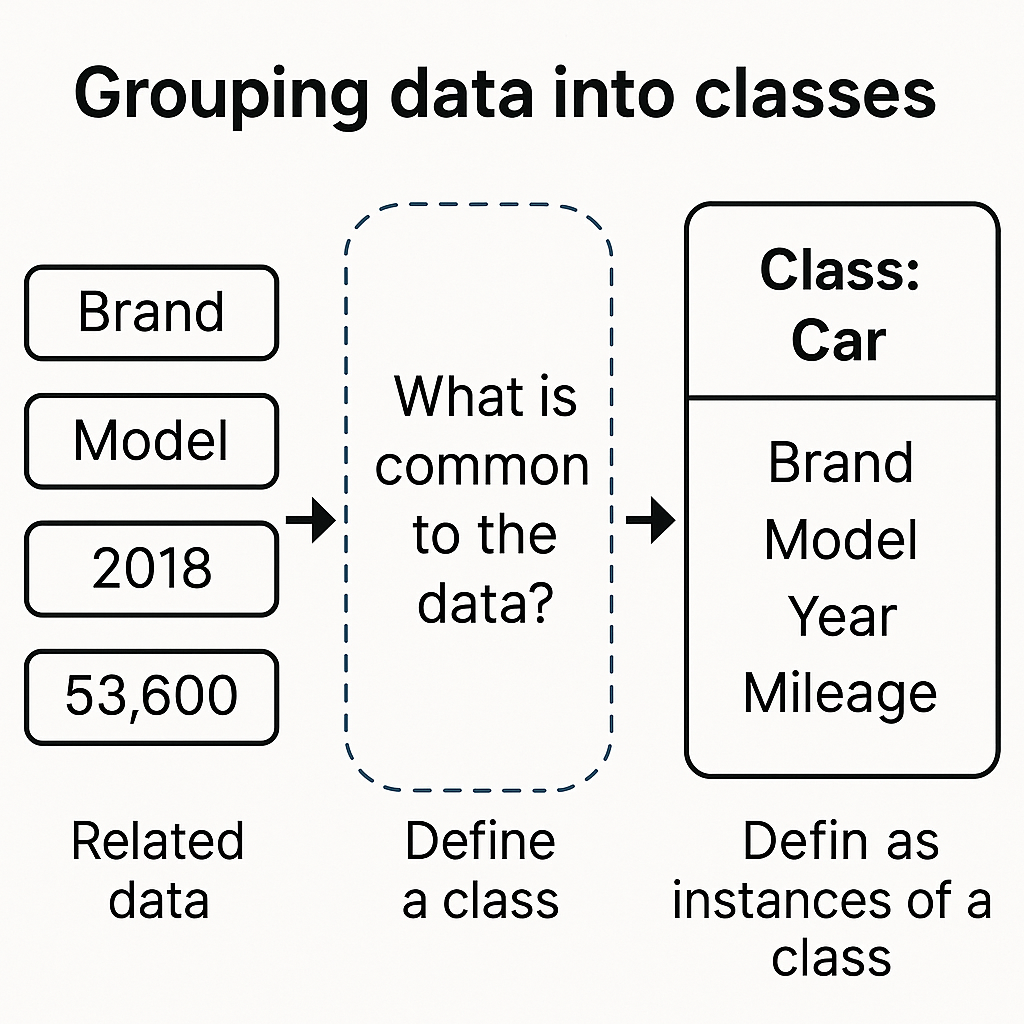
\includegraphics[width=\textwidth]{images/oven_abstraction_example.png}
\end{center}

